---
title: Cohen実数はSuslin木を付加する
date: 2016/11/25 15:00:00 JST
author: 石井大海
description: Shelahは実数の集合の性質に関する記念碑的論文 [@Shelah:1984] において滅茶苦茶いろいろな事を示していて本当にヤバいんですが,その中で一節割いて「Cohen実数を付加するとSuslin木も足される」という事を示しています.原論文における構成は結構煩雑に見えますが,後にTodorčevićは彼の発明した\emph{minimal walk}の手法を用いて自然で比較的簡単な構成を与えました.minimal walkの手法はAronszajn木の構成にも使えますが,これとCohen実数を単に合成してやる事でSuslin木が得られるのです.本稿ではこの方法について(強制法の基礎理論は別にして)証明します.
latexmk: -lualatex
tag: 数学,数理論理学,集合論,無限組合せ論,極小歩,minimal walk,木,Suslin木,Aronszajn木,強制法,Cohen実数
katex: true
---
\RequirePackage{luatex85}
\documentclass[a4j]{ltjsarticle}
\usepackage[hiragino-pron]{luatexja-preset}
\usepackage{mystyle}
\usepackage{luatexja-otf}
\usetikzlibrary{matrix,arrows,shapes,backgrounds,positioning}
\usetikzlibrary{arrows,calc,decorations.pathmorphing}
\usetikzlibrary{decorations.markings,intersections,decorations.pathreplacing}
\usepackage{dsfont}
\usepackage{luatexja-ruby}
\DeclareMathAlphabet{\mathrsfs}{U}{rsfso}{m}{n}
\renewcommand{\mathscr}[1]{\mathup{\mathrsfs{#1}}}
\usepackage{fixme}
\usepackage[bookmarksnumbered,pdfproducer={LuaLaTeX},%
            luatex,psdextra,pdfusetitle,pdfencoding=auto]{hyperref}
\usepackage[backend=biber, style=math-numeric]{biblatex}
\addbibresource{myreference.bib}
\renewcommand{\emph}[1]{\textsf{\textgt{#1}}}
\newcommand{\SH}{\mathreg{SH}}
\newframedtheorem{conjecture}{予想}

\title{Suslin木,Cohen実数,Minimal Walk}
\date{}
\author{石井大海}

\usepackage{amsmath}
\begin{document}

\maketitle
\begin{abstract}
 Shelahは実数の集合の性質に関する記念碑的論文~\cite{Shelah:1984}において滅茶苦茶いろいろな事を示していて本当にヤバいんですが,その中で一節割いて「Cohen実数を付加するとSuslin木も足される」という事を示しています.
 原論文における構成は結構煩雑に見えますが,後にTodor\v{c}evi\'{c}~\cite{Todorcevic:1987fj}は彼の発明した\emph{minimal walk}の手法を用いて自然で比較的簡単な構成を与えました.
 minimal walkの手法はAronszajn木の構成にも使えますが,これとCohen実数を単に合成してやる事でSuslin木が得られるのです.
 本講演では,まず背景となる話題を紹介した後,これまでにやってきた強制法の応用例としてこの手法を紹介します.
\end{abstract}

\section{背景:直線の姿を予想する──Suslin予想}
現代的な一般位相空間論では,よく\emph{可分性}が問題になりますが,初期にそれと並んでよく採り上げられていたのが\emph{可算鎖条件} (countable chain condition; c.c.c.)でした:

\begin{definition}
 \begin{itemize}
  \item 位相空間$X$が\emph{可分}$\defs$ $X$は稠密な可算部分集合$D$を持つ.
  \item 位相空間$X$が\emph{可算鎖条件}(countable chain condition; \emph{c.c.c.})を持つ$\defs$
        $X$の互いに交わらない開集合の族の濃度は高々可算.
        言い換えれば,$X$の非可算個の開集合から成る任意の族$\Braket{U_\alpha | \alpha < \omega_1}$に対し,$U_\alpha \cap U_\beta \neq \emptyset$となる$\alpha < \beta < \omega_1$が必ず存在する.
 \end{itemize}
\end{definition}
任意の擬順序集合$\mathbb{P}$はその開集合代数$\mathcal{O}_{\mathbb{P}}$に稠密に埋め込めるので,擬順序に関するc.c.c.は位相空間のc.c.c.の特別な場合になっています.

位相空間が可分であればc.c.c.を持つことはすぐにわかります:

\begin{lemma}
 位相空間$X$が可分ならc.c.c.を持つ.
\end{lemma}
\begin{proof}
 $D = \Set{d_n \in X | n < \omega}$を$X$の可算稠密部分集合とし,$\Braket{U_\alpha | \alpha < \omega_1}$を$X$の開集合から成る族とする.
 このとき,$D$の稠密性から各$\alpha < \omega_1$に対し,$d_n \in U_\alpha$となる$n < \omega$が取れる.
 そこで$D_n \defeq \Set{\alpha < \omega_1 | d_n \in U_\alpha}$とおけば,$\omega_1$の正則性から少なくとも一つの$n$について$D_n$は非可算でなくてはならない.
 よってそこから$\alpha< \beta \in D_n$を取れば$d_n \in U_\alpha \cap U_\beta \neq \emptyset$. \qed
\end{proof}

では逆はどうか?というと,$2^\kappa$に積位相を入れたものが反例になります:
\begin{lemma}
 $\kappa > 2^\omega$とするとき,$2^\kappa$に直積位相を入れた空間はc.c.c.だが可分ではない.
\end{lemma}
\begin{proof}
 まずc.c.c.を示そう.
 基本開集合から成る任意の族$\Braket{U_\alpha | \alpha < \omega_1}$を適当に取ってきて,
 交わりを持つ二元が取り出せれば良い.
 まず,各$U_\alpha$は$S_\alpha \in [\kappa]^{<\aleph_0}$と$U^\alpha_\beta \subsetneq 2$があって,$U_\alpha = \prod_{\beta \in S_\alpha} U^\alpha_\beta \times \prod_{\kappa \setminus S_\alpha} 2$の形で書けていました.
 この$S_\alpha$を$U_\alpha$の\emph{台}(\emph{support})と呼びましょう.
 各$U_\alpha$はその台$S_\alpha$上での所属関係だけしか気にしない,という訳です.
 また,直積成分$2$には離散位相が入っているので,各$U_\alpha$は関数$h_\alpha : S_\alpha \to 3$と同一視出来ることに注意しましょう.

 そこで$\omega_1$の部分集合の族$\Braket{S_\alpha | \alpha < \omega_1}$を取ると,$\Delta$-システム補題から$X \in [\omega_1]^{\aleph_1}$で$\Braket{S_\alpha | \alpha \in X}$が$\Delta$-システムを成すものが取れます.
 即ち,$S \in [\omega_1]^{<\aleph_0}$があって,どんな$\set{\alpha, \beta} \in [X]^{\aleph_1}$に対しても,$S_\alpha \cap S_\beta = S$となるようなものが取れます.
 これはどういう事かというと,$X$から相異なる$\alpha, \beta$を取ってきた時に,条件が競合する場所は$S$上だけになっている,という事です.
 この時,$S$上での基本開集合の組み合わせは高々$3^{|S|} < \aleph_0$通りしかないのに対し,$S_\alpha$たちは$\omega_1$個もありますから,正則性から適当な$Y \in [X]^{\aleph_1}$が取れて,$\alpha, \beta \in Y$なら$U^\alpha_\xi = U^\beta_\xi \;(\xi \in S)$となるように出来ます.
 よって,$\alpha, \beta \in Y$とすれば,$U_\alpha \cap U_\beta \neq \emptyset$となります.
 以上より$2^\kappa$はc.c.c.を満たします.

 最後に可分でない事を見ましょう.
 可算列$\Braket{x_n \in 2^\kappa | n < \omega}$を任意に取って,これと交わらない空でない開集合を与えれば良いでしょう.
 この時,$\xi < \kappa$に対して,列$\Braket{x_n(\xi) | n < \omega}$の総数は高々$2^\omega$個ですから,$2^\omega < \kappa$なので鳩ノ巣原理から$\xi < \eta < \kappa$で任意の$n < \omega$に対して$x_n(\xi) = x_n(\eta)$となるものが取れます.
 そこで,$W \defeq \Set{x \in 2^\kappa | x(\xi) = 0, x(\eta) = 1}$とおけば,$W$は空でない開集合です.
 すると,$\xi, \eta$の取り方から任意の$n < \omega$に対し$x_n(\xi) = x_n(\eta)$が成り立つので,$x_n \in W$となります. \qed
\end{proof}

では順序位相に限定した場合はどうでしょうか?
実数直線$\R$は可分な全順序位相空間として有名です:

\begin{fact}
 $(X, <)$を次を満たす全順序位相空間(i.e. $x, y \in X \cup \set{\pm \infty}$に対し区間$(x, y)$が生成する位相)とする:
 \begin{enumerate}
  \item $(X, <)$は端点を持たない稠密全順序,
  \item $(X, <)$は位相空間として連結で可分.
 \end{enumerate}
 この時,$(X, <) \simeq (\R, <)$.
\end{fact}

Suslinは「可分をc.c.c.で置き換えても同じ事が言える」と予想しました:
\begin{conjecture}[Suslin予想$(\SH)$]
 c.c.c.だが可分でない全順序位相空間(\emph{Suslin直線})は存在しない.
\end{conjecture}

連結とか稠密とかが落ちていますが,適当に完備化とかを取れば同値になります.

これはまだ位相空間論的な概念ですが,木の概念を使うことで集合論的に言い換えることが出来ます:

\begin{definition}
 \begin{itemize}
  \item $T \subseteq \power{<\alpha}{X}$が\emph{木}(\emph{tree}) $\defs$ $T$は始切片について閉じている:$\forall t \in T \: \forall n < \lh(t)\: t\restr n \in T$.
  \item $C \subseteq T$が\emph{鎖}$\defs$ $C$は$(T, \subseteq)$の全順序部分集合.
  \item $A \subseteq T$が\emph{反鎖}$\defs$任意の$s, t \in A$, $s \neq t$に対し$s \nsubseteq t$かつ$t \nsubseteq s$.
  \item $x \in T$に対し,$\rank_T(x) \defeq \sup\Set{ \rank_T(y) + 1 | y \in T, y \subsetneq x}$を$x$の$T$における\emph{ランク}と言う.
  \item $\height(T) \defeq \sup_{x \in T} (\rank_T(x) + 1)$を$T$の\emph{高さ}と呼ぶ.
  \item $T_\alpha \defeq \Set{x \in T | \rank_T(x) = \alpha}$.
  \item $C \subseteq T$が\emph{共終鎖}$\defs$ $C$は$T$の鎖で,$\forall \alpha < \height(T)\: T_\alpha \cap C \neq \emptyset$.
  \item $T$が\emph{$\kappa$-木}$\defs$ $\height(T) = \kappa$かつ任意の$\alpha < \kappa$に対し$|T_\alpha| < \kappa$.
  \item $T$が\emph{$\kappa$-\ruby{Aronszajn}{アロンシャイン}木}$\defs$ $T$は$\kappa$-木で鎖は全て濃度$\kappa$未満.
        $\omega_1$-Aronszajn木を\emph{Aronszajn木}と呼ぶ.
  \item $T$が\emph{($\kappa$-)Suslin木}(または\emph{Souslin木})$\defs$ $T$は($\kappa$-)Aronszajn木で,$T$の反鎖は濃度$\kappa$未満.

 \end{itemize}
\end{definition}

\begin{fact}
 Suslin直線の存在とSuslin木の存在は同値
\end{fact}
\begin{proof}
 See \S III.5 of Kunen~\cite{Kunen:2011}.
\end{proof}

よって$\SH$はSuslin木があるかないか,という問題に帰着されます.
実は$\SH$は$\ZFC$上独立であることがわかっています.
今回扱うのは特に$\ZFC+\neg \SH$の無矛盾性,つまり「Suslin木がある」方向の結果です.

\section{Cohen実数はSuslin木を付加する}

\begin{theorem}[Shelah~\cite{Shelah:1984}]
 Cohen強制法$\mathbf{C}$はSuslin木を付加する.
\end{theorem}

まず次の補題を認める:

\begin{lemma}
 次を満たす列$\Braket{e_\alpha | \alpha < \omega_1}$が存在する:
 \begin{enumerate}
  \item \label{item:e-fin-one}有限対一:各$\alpha$について$e_\alpha : \alpha \to \omega$は有限対一
        (i.e. $\Set{ \beta < \alpha | e_\alpha(\beta) = n }$は有限),
  \item \label{item:e-homog}斉一性:各$\alpha < \beta < \omega_1$に対し,$\left|\Set{\xi < \alpha | e_\alpha(\xi) \neq e_\beta(\xi)}\right| < \aleph_0$.
 \end{enumerate}
\end{lemma}

これを認めた上で先に定理1を示す.
まず,このような列からAronszajn木が作れることを見ておく:

\begin{lemma}
 補題1のような$\Braket{e_\alpha | \alpha < \omega_1}$に対し,$T \defeq \Set{e_\alpha \restr \beta | \beta \leq \alpha < \omega_1}$はAronszajn木となる.
\end{lemma}
\begin{proof}
 まず$T$が$\omega_1$-木となることを見る.
 $T$の第$\alpha$レベルは$T_\alpha \defeq \Set{ e_\beta \restr \alpha | \beta \in [\alpha, \omega_1)}$と書け,明らかに$e_\alpha \in T_\alpha$なので,$\mathop{\mathreg{ht}}(T) = \omega_1$は良い.
 また,条件~\ref{item:e-homog}から$t \in T_\alpha$なら$|\Set{\xi < \alpha | t(\xi) \neq e_\alpha(\xi)}| < \aleph_0$なので,結局$|T_\alpha| \leq [\alpha]^{<\aleph_0} \times \omega = \aleph_0$より$T_\alpha$は可算.
 以上より$T$は$\omega_1$-木である.

 最後に$T$が非可算鎖を持たないことを示そう.
 そこで$C \subseteq T$が非可算鎖だったとすると,共終性から$\bigcup C: \omega_1 \to \omega$となる.
 しかし,条件~\ref{item:e-fin-one}より$C$の各元は有限対一写像なので,その貼り合わせである$\bigcup C$は$\omega_1$から$\omega$への有限対一写像となってしまうので矛盾. \qed
\end{proof}


\begin{proof}[Proof of Theorem 1]
 $V$で補題1の性質を満たす$\Braket{e_\alpha | \alpha < \omega_1}$を取り,$r$を$V$上のCohen実数とする.
 この時,Cohen強制法はc.c.c.を満たすので$e_\alpha$たちは$V[r]$上でも依然として補題の条件を満たすことに注意する.
 この時,$T(r) \defeq \Set{r \circ e_\alpha \restr \beta | \beta < \alpha < \omega_1}$ が$V[r]$でSuslin木となる事を示そう.

 まず,上と同様に$T_\alpha(r) = \Set{ r \circ e_\beta \restr \alpha | \beta \in [\alpha, \omega_1)}$であり,前の補題と同様にして$T(r)$が$\omega_1$-木になることが従う.

 次に$T(r)$は非可算反鎖も可算反鎖も持たないことを示そう.
 $V[r]$で$\mathcal{A} = \Set{ r \circ t_\alpha | \alpha < \omega_1} \in [T(r)]^{\aleph_1}$を任意に取り,これが両立する二元も両立しない二元も含むことを示せばよい.
 簡単の為,以下$\alpha < \beta \implies \lh(t_\alpha) \leq \lh(t_\beta)$であるとしよう.
 のちほど稠密集合を使った議論をしたいので,まずは$\Braket{t_\alpha | \alpha < \omega_1}$が$V$に列として入っているとして良いことを見よう.
 そこで$X_p \defeq \Set{t_\alpha | p \Vdash^{V}_{\mathbf{C}} \quoted{\dot{r} \circ t_\alpha \in \dot{\mathcal{A}}}}$とおけば,各$p \in \mathbf{C}$について$X_p \in V$が成り立つ.
 このとき,$\Set{t_\alpha | \alpha < \omega_1} = \bigcup_{p \subset r} X_p$であり,$p \subset r$なる$p$は可算個しかないので,少なくとも一つの$X_p$は非可算となる.
 よって,最初からこの$X_p$の元に範囲を取り直せば,$\Set{t_\alpha | \alpha < \omega_1} \in V$であるとしてよい.

 
 斉一性の条件~\ref{item:e-homog}より,各$t_\alpha$が両立するか否かは,その有限桁だけ見てやればよい.
 そこで,$t_\beta, t_{\beta'}$の値が一致する範囲を表す記号を導入する:
 \[
  \Delta(\beta, \beta') \defeq \min\Set{ n < \omega | \forall \xi < \beta \: [t_\beta(\xi), t_{\beta'}(\xi) \geq n \implies t_\beta(\xi) = t_{\beta'}(\xi)]}.
 \]
 この記号を使えば,$\mathcal{A}$が反鎖でも鎖でもない事を示すには,以下の二つの集合がそれぞれ$\mathbf{C}$で稠密となることが示せればよい:
 \begin{align*}
  E &\defeq \Set{p \in \mathbf{C} | \exists \beta < \beta' < \omega_1 \: [p \circ t_\beta = p \circ t_{\beta'} \restr \beta, \Delta(\beta, \beta') \leq \lh(p)] },\\
  D &\defeq \Set{p \in \mathbf{C} | \exists \beta < \beta' < \omega_1 \: [p \circ t_\beta \neq p \circ t_{\beta'} \restr \beta, \Delta(\beta, \beta') \leq \lh(p)]}.
 \end{align*}
 実際,$E$が$\mathbf{C}$で稠密なら,$V[r]$において$p \subset r$で$p \in E$となるものが取れ,
 証拠となる$\beta < \beta' < \omega_1$を取れば$p \circ t_\beta = p \circ t_{\beta'} \restr \beta$であり,$\Delta(\beta, \beta') \leq \lh(p)$より$r \circ t_\beta = r \circ t_{\beta'} \restr \beta$となり,これが$\mathcal{A}$の両立する二元となる.
 同様に$D$に属す$p \subseteq r$が取れれば,証拠となる$\beta < \beta'$について$r \circ t_{\beta} \perp r \circ t_{\beta'}$となるので,これら二元は両立しない.

 あとは$E$, $D$がそれぞれ稠密となる事がわかればよい.
 そこで$p \in \power{n}{\omega}$を固定する.
 適当な$t_\alpha, t_\beta$をとってきてしまうと,$p$で決まっている範囲で既に$p \circ t_\alpha$と$p \circ t_\beta$が異なってしまうかもしれない.
 そうした場合を排除するために$t_\alpha$たちを取り直そう.
 まず,$n$未満の値を取る$\xi < \omega_1$が$t_\alpha, t_\beta$とで一致するような$\alpha < \beta$が非可算個とれることを見よう.

 そこで$X_\alpha \defeq \Set{\xi < \alpha | t_{\alpha}(\xi) < n\; (= \lh(p))}$と置けば,各$t_\alpha$が有限対一写像である事より$X_\alpha$は有限集合となる.
 よって$\Delta$-システム補題を$\Set{X_\alpha \in [\omega_1]^{<\aleph_0} | \alpha < \omega_1}$に適用すれば,$Z \in [\omega_1]^{\aleph_1}$と$S \in [\omega_1]^{<\aleph_0}$で$\forall \set{\alpha, \alpha'} \in [Z]^2\: X_\alpha \cap X_{\alpha'} = S$となる物が取れる.
 この時,$t_\alpha \restr S$の候補は可算個しかないので,鳩ノ巣原理から$\forall \set{\alpha, \alpha'} \in [Z]^2 \: t_\alpha \restr S = t_{\alpha'} \restr S$となるように$Z$を取り直せる.
 一々$Z$と書くのは面倒なので,そもそも始めから$\mathcal{A}$はこのように取れているとして以下議論を進めていく.
 そこで,$\alpha_1 < \alpha_2 < \omega_1$を取り,$p$を長さ$m \defeq \Delta(\alpha_1, \alpha_2)$まで拡張する事を考えよう.

 まず$E$に属する元を取りたい.
 $k = t_{\alpha_1}(\xi) \neq t_{\alpha_2}(\xi) = \ell$となるような$k, \ell$が共に$n$以上であれば,
 $q(k) = 0$によって潰せば良い.
 もし少なくとも一方が$n$未満であれば,同じ行き先に行くように潰してやればよい.
 \[
  q(k) \defeq \begin{cases}
               p(\ell) & \exists \xi < \alpha_1 \: k = t_{\alpha_i}(\xi) \wedge \ell = t_{\alpha_{1-i}}(\xi) < n\\
               0 & \text{otherwise}.
              \end{cases}
 \]
 各$t_\alpha$たちが単射である事に注意すれば,定義から$q \circ t_{\alpha_1} = q \circ t_{\alpha_2} \restr \alpha_1$であり$q \leq p$, $\lh(q) = \Delta(p, q)$である.

 最後に$D$に入るように延ばせる事を見る.
 この時,相異なる$\alpha < \alpha' < \omega_1$で$n \leq \Delta(\alpha, \alpha')$を満たすものが取れる.
 なぜなら,もし仮に任意の$\alpha, \alpha' \in Z$に対し$\Delta(\alpha, \alpha') < n$となるのであれば,適当な$\alpha_0 < \omega_1$を取って,
 \[
  e'_{\beta(\alpha)}(\xi) \defeq \begin{cases}
                                  e_{\beta(\alpha_0)}(\xi) & e_{\beta(\alpha)}(\xi) < n\\
                                  e_{\beta(\alpha)}(\xi)   & \text{otherwise}
                                 \end{cases}
 \]
 と定めてやれば,族$\Braket{e'_\alpha | \alpha < \omega_1}$は依然として仮定~\ref{item:e-fin-one}, \ref{item:e-homog}を満たす.
 しかし,この時$\Set{e'_{\beta(\alpha)} \restr \alpha | \alpha \in W}$は$\Set{e'_\alpha \restr \beta | \alpha, \beta < \omega_1}$の鎖となり,補題2に反する.
 よって,$\Delta(\alpha_0, \alpha_1) \geq n$を満たす$\alpha_0 < \alpha_1 < \omega_1$が存在する.
 そこで$t_{\alpha_i}(\xi)$の少なくとも一方が$n$以上となるような$\xi < \beta$を取る.
 この時,$k \in [n, \Delta(\alpha_0, \alpha_1)]$に対し,
 \[
  q(k) \defeq
  \begin{cases}
   p(t_{\alpha_{1-i}}(\xi)) + 1 & (t_{\alpha_i}(\xi) = k, t_{\alpha_{1-i}}(\xi) < n)\\
   k & (\ow)
 \end{cases}
 \]
 とおけば$q \circ t_\beta \neq q \circ t_{\beta'} \restr \beta$.

 以上より$D$, $E$は$\mathbf{C}$で稠密となり,$V[r] \models \quoted{T_r: \text{Suslin}}$が言えた. \qed
\end{proof}

\section{斉一列$e_\alpha$の構成}
最後に補題1を満たす$\Braket{e_\alpha | \alpha < \omega_1}$をTodor\v{c}evi\'{c}によるwalkの手法を用いて構成する.

\begin{definition}
 \begin{itemize}
  \item 以下を満たす$\Braket{C_\alpha | \alpha < \omega_1}$を\emph{$C$-列}と呼ぶ:
  \begin{enumerate}
   \item $C_{\alpha + 1} \defeq \set{\alpha}$,
   \item $C_\gamma \subseteq \gamma$ : cofinal in $\gamma$, $\otp(C_\gamma) = \omega$.
  \end{enumerate}
        $C$-列は明らかに存在するので,以下一つ固定する.
  \item $\alpha < \beta < \omega_1$に対し,$\beta$から$\alpha$への\emph{step}とは$\min(C_\beta \setminus \alpha) < \beta$の事.
  \item $\beta$から$\alpha$への\emph{walk}とは次で定まる$\Braket{s^\beta_\alpha(i) | i < \omega}$の事:
        \[
         s^{\beta,\alpha}_0 \defeq \beta,\qquad
         s^{\beta,\alpha}_{i+1} \defeq \min(C_{s^{\beta,\alpha}_i} \setminus \alpha).
        \]
        walkは順序数の真の減少列なので有限長で止まる.
        定義より$\forall i \: s^{\beta,\alpha}_i \geq \alpha$であり,$C$-列の取り方より$s^{\beta,\alpha}_i > \alpha$なら$s^{\beta,\alpha}_{i+1}$は必ず定まるので,特に最終的に$\alpha$と一致する.
  \item $\rho_1(\alpha, \alpha) = 0, \rho_1(\alpha, \beta) \defeq \max\{\ |C_\beta \cap \alpha|, \rho_1(\alpha, s^{\beta,\alpha}_1)\ \}$
        により関数$\rho_1$を定める.$\rho_1(\alpha, \beta)$を\emph{$\beta$から$\alpha$へのwalkの最大重み(maximal weight)}と呼ぶ.
 \end{itemize}
\end{definition}

定義だけだとわかりづらいと思うので,$\alpha < \beta < \omega_1$を固定しよう.
記号が重いので,$\beta_i \defeq s^{\beta,\alpha}_i$と略記することにすれば,以下のように図示出来る:
\begin{center}
 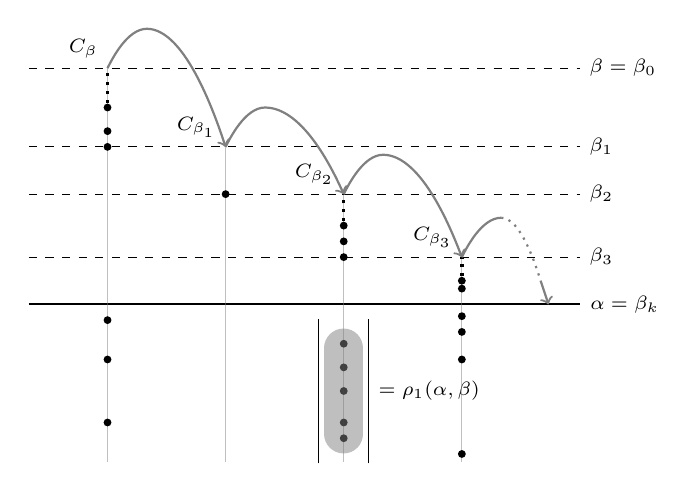
\begin{tikzpicture}[every node/.style={font=\scriptsize}]
  \path[dashed,draw] (-5, 5) -- ++ (7, 0) node[right]{$\beta = \beta_0$};
  \path[draw, thick] (-5, 2) -- ++ (7, 0) node[right]{$\alpha = \beta_k$};
  \coordinate[label=above left:{$C_\beta$}]  (s0) at (-4,5);
  \path[gray,opacity=.5,draw]
    (s0) -- (s0 |- 0, 0);

  \foreach \i/\y in {0/4 , 1/4.2, 2/4.5} {
    \node[fill=black,inner sep=1pt,circle] (C-0-\i) at (s0 |- 0, \y) {} ;
  };
  \foreach \i/\y in {0/.5 , 1/1.3, 2/1.8} {
    \node[fill=black,inner sep=1pt,circle] (W-0-\i) at (s0 |- 0, \y) {} ;
  };
  \path[dotted, draw, very thick] (C-0-2) -- (s0);

  \coordinate[label={above left:$C_{\beta_1}$}] (s1) at (C-0-0 -| -2.5,0);
  \path[dashed,draw] (-5, 0 |- s1) -- (2, 0 |- s1) node[right]{$\beta_1$};
  \path[gray,opacity=.5,draw]
    (s1) -- (s1 |- 0, 0);
  \node[fill=black, inner sep=1pt, circle]
    (C-1-0) at ($(s1)-(0,.6)$) {};

  \coordinate[label={above left:$C_{\beta_2}$}] (s2) at (C-1-0 -| -1,0);
  \path[dashed,draw] (-5, 0 |- s2) -- (2, 0 |- s2) node[right]{$\beta_2$};
  \path[gray,opacity=.5,draw]
    (s2) -- (s2 |- 0, 0);
  \foreach \i/\y in {0/2.6,1/2.8 , 2/3} {
    \node[fill=black,inner sep=1pt,circle] (C-2-\i) at (s2 |- 0, \y) {} ;
  };
  \foreach \i/\y in {0/.3 , 1/.5, 2/.9, 3/1.2, 4/1.5} {
    \node[fill=black,inner sep=1pt,circle] (W-2-\i) at (s2 |- 0, \y) {} ;
  };
  \path[dotted, draw, very thick] (C-2-2) -- (s2);

  \path[draw=gray,opacity=.5,fill=gray,line cap=round,line width=5mm]
    (W-2-0) --  (W-2-4);
  \path[draw]
    ($(W-2-0.south west)-(2.8mm,2.8mm)$) -- ($(W-2-4.north west)+(-2.8mm,2.8mm)$)
  ;
  \path[draw]
    ($(W-2-0.south east)+(2.8mm,-2.8mm)$) --
    node[right,black] {$= \rho_1(\alpha, \beta)$}
    ($(W-2-4.north east)+(2.8mm,2.8mm)$)
  ;

  \coordinate[label={above left:$C_{\beta_3}$}] (s3) at (C-2-0 -| .5,0);
  \path[dashed,draw] (-5, 0 |- s3) -- (2, 0 |- s3) node[right]{$\beta_3$};
  \path[gray,opacity=.5,draw]
    (s3) -- (s3 |- 0, 0);
  \foreach \i/\y in {0/2.2,1/2.3} {
    \node[fill=black,inner sep=1pt,circle] (C-3-\i) at (s3 |- 0, \y) {} ;
  };
  \foreach \i/\y in {0/.1 , 1/1.3, 2/1.65, 3/1.85} {
    \node[fill=black,inner sep=1pt,circle] (W-3-\i) at (s3 |- 0, \y) {} ;
  };
  \path[dotted, draw, very thick] (C-3-1) -- (s3);

  \path[draw, gray, thick, ->]
    (s0) parabola bend +(.5,.5) (s1);
  \path[draw, gray, thick, ->]
    (s1) parabola bend +(.5,.5) (s2);
  \path[draw, gray, thick, ->]
    (s2) parabola bend +(.5,.5) (s3);
  \path[draw, gray, thick]
    (s3) parabola bend ++(.5,.5) ++ (.5,.5) coordinate  (interr);
  \path[draw, dotted, gray, thick]
    (interr) parabola (1.5,2.3) coordinate (batsu);
  \path[draw, gray, thick,->]
    (batsu) -- (1.6,2);
 \end{tikzpicture}
\end{center}

$\beta$から$\alpha$に向けて$\Braket{C_\xi | \xi < \omega_1}$を梯子に使って降りていくようなイメージである.
特に,各$C_\xi$は$\omega$-型に取ってあるので,途中の$\alpha$で切ったら必ず有限で切れるようになっている.
$\rho_1$はこの$\alpha$未満の有限の端数の所に注目して,一番長い所の長さを持ってきた物である.
そして,この$\rho_1$が補題1の列を作る本質的な素になっている.

\begin{lemma}
 \begin{enumerate}
  \item $\rho_1(-, \beta)$は有限対一写像:任意の$n < \omega$に対し$|\Set{\xi < \beta | \rho_1(\xi, \beta) = n}| < \aleph_0$,
  \item $\rho_1$は斉一的(coherent):任意の$\beta < \alpha < \omega_1$に対し$|\Set{\xi < \beta | \rho_1(\xi, \beta) \neq \rho_1(\xi, \alpha)}| < \aleph_0$.
 \end{enumerate}
\end{lemma}
\begin{proof}
 \begin{enumerate}
  \item 任意の$A \in [\beta]^{\aleph_0}$と$n < \omega$に対し$n < \rho_1(\xi, \beta)$を満たす$\xi \in A$の存在を示せば良い.
        特に,$|C_\alpha \cap \xi| > n$を満たす$\xi \in A$が取れるのなら自明なので,$\forall \xi \in A \: |C \cap \xi| \leq n$としよう.

        $\beta$について帰納法で示す.

        $\alpha \defeq \sup A$と置く.
        $\alpha = \beta$ならば,十分大きな$\xi \in A$で$\rho_1(\xi, \beta) \geq |C_\beta \cap \xi| > n$を満たすものがある.

        そこで$\alpha < \beta$の場合を考える.
        $\omega$の正則性から,特に$|C_\beta \cap \xi| = n$が任意の$\xi \in A$に対して成立しているとして良く,この時$\eta \defeq s^{\beta}_\xi(1) = \min(C_\beta \setminus \xi)$は$\xi \in A$に依らず常に一定の値を取り,特に$\alpha = \sup A \leq \eta$が成り立つ.
        この時,各$\xi \in A$に対し,
        \[
         \rho_1(\xi, \beta) = \max \set{ n, \rho_1(\xi, \eta) }
        \]
         そこで帰納法の仮定を$\eta$と$A \subseteq \eta$に適用すれば,$\xi \in A$で$n < \rho_1(\xi, \eta)$を満たすものが取れる.すると,
        \[
         \rho_1(\xi, \beta) = \max\set{n, \rho_1(\xi, \eta)} > n.
        \]

        よって$\rho_1$は有限対一.
  \item $\alpha$についての帰納法で示す.

        $\beta < \alpha$と$A \in [\beta]^{\aleph_0}$を任意に取って,$\xi \in A$で$\rho_1(\xi, \beta) = \rho_1(\xi, \alpha)$を満たすものを取れれば良い.
        適切に$A$を縮めれば,$\otp A = \omega$としても一般性を失わない.
        $\gamma \defeq \sup A \leq \beta$, $\eta \defeq s^{\alpha,\gamma}_1$, $n \defeq |C_\alpha \cap \gamma|$とおく.
        上の結果から$\rho_1$は有限対一なので,
        \[
         B \defeq \Set{\xi \in A | \xi > \max(C_\alpha \cap \gamma), \rho_1(\xi, \eta) > n }
        \]
        とおけば$|A \setminus B| < \aleph_0$.
        $\xi \in B \subseteq A$をとれば,$\sup A = \gamma \geq \xi > \max(C_\alpha \cap \gamma)$より$C_\alpha \cap \xi = C_\alpha \cap \gamma$および$C_\alpha \setminus \xi = C_\alpha \setminus \gamma$.
        以上を踏まえれば,
        \begin{align*}
         \rho_1(\xi, \alpha) &= \max \{\ |C_\alpha \cap \xi|, \rho_1(\xi, s^{\alpha,\xi}_1) \ \}\\
         &= \max \{\ \underbrace{|C_\alpha \cap \gamma |}_{= n}, \underbrace{\rho_1(\xi, \eta)}_{> n} \ \} = \rho_1(\xi, \eta).
        \end{align*}
        ここで,$\eta = \beta$なら$\rho_1(\xi, \alpha) = \rho_1(\xi, \beta)$となるので適当に$\xi \in B$を取ればそれが求めるものである.
        もし$\eta < \beta$であれば,$B$に帰納法の仮定が使え,$\xi \in B$で$\rho_1(\xi, \eta) = \rho_1(\xi, \beta)$を満たすものが取れ,上の議論と合わせて$\rho_1(\xi, \alpha) = \rho_1(\xi, \beta)$となる. \qed
 \end{enumerate}
\end{proof}

\section{折角なので$\SH$の無矛盾性の概要を}
こうしてSuslin予想を打ち砕く方向の構成は出来ました.
では逆に$\SH$を成り立たせる,つまり「Suslin木がない」状況を実現するにはどうすればいいでしょうか?
まず,Suslin木のうち性質の良い木だけ考えればよい,ということを見ましょう:

\begin{definition}
 $\kappa$-木$T$が\emph{well-pruned} $\defs$ どんな$s \in T$に対しても$t \supsetneq s$となる$t \in T$が$\kappa$-個存在.
\end{definition}

\begin{lemma}
 $\kappa$-Suslin木が存在するなら,well-prunedな$\kappa$-Suslin木も存在.
\end{lemma}
\begin{proof}
 そういう頂点だけ集めてくればいいだけ. \qed
\end{proof}

例えば,一つSuslin木が与えられた時に,それを壊すだけなら簡単です:

\begin{lemma}
 $T$をwell-prunedな$\kappa$-木とする.この時,$s \leq t \defs s \supseteq t$により$(T, \supseteq)$を擬順序と見做す.
 この時,$G$を$V$上の$T$-ジェネリックフィルターとすると,$G$は$T$の濃度$\kappa$の鎖.

 特に,$T$がAronszajn木(Suslin)なら$V[G]$において$T$はAronszajn(Suslin)ではない.
\end{lemma}
\begin{proof}
 $T$は$\kappa$-木で,しかもwell-prunedなので,各$\alpha < \kappa$に対し,$D_\alpha \defeq \Set{ s \in T | \rank_T(s) > \alpha}$は$T$で稠密.
 よって,$G$は任意の$\alpha < \kappa$に対して$G \cap D_\alpha \neq \emptyset$.
 また,$G$の任意の二元は両立し,$G \subseteq X^{<\alpha}$なので$G$は鎖.
 よって$G$は濃度$\kappa$の$T$の鎖. \qed
\end{proof}

よって一つ具体的に$T$が与えられていれば,$T$で強制する事によって$T$のSuslin性を壊すことが出来ます.

なので,Suslin木を全部一列に並べておいて順に強制してやれば……という発想に至るのは自然な事です.
しかし,問題となるのは,Suslin木で強制した事によって別のSuslin木が付加されている可能性がある,ということです.
そういった状況下で,「途中で増えるかもしれない物の帳尻を最終的に合わせる」手法を\emph{bookkeeping論法}といい,集合論では常套手段になっています.
まず,Suslin木は強制法としてc.c.c.持ち,特に任意の基数を保つことに注意しましょう.

これを踏まえて,全てのSuslin木を殺す強制法を考えましょう.
そのためには,「いちど強制拡大した後に追加される強制法で頑張る」という方法が必要になります.
これを定式化したものが\emph{反復強制法}です:

\begin{definition}
 $\mathbb{P}$を擬順序とする.
 \begin{itemize}
  \item $\dot{\mathbb{Q}} = (\dot{\mathbb{Q}}, \dot{\leq}_{\mathbb{Q}}, \dot{\mathds{1}}_{\mathbb{Q}})$が\emph{擬順序の$\mathbb{P}$-名称}$\defs$ $\mathbb{P} \Vdash \quoted{\dot{\mathbb{Q}} : \text{擬順序}}$.
  \item $\dot{\mathbb{Q}}$を擬順序の$\mathbb{P}$-名称とする.
        このとき,$\mathbb{P}$と$\dot{\mathbb{Q}}$の\emph{二段階反復}$\mathbb{P} \ast \dot{\mathbb{Q}}$を次で定める:
        \begin{gather*}
         \mathbb{P} \ast \dot{\mathbb{Q}} \defeq \Set{(p, \dot{q}) | p \in \mathbb{P}, \mathds{1} \Vdash_{\mathbb{P}} \quoted{\dot{q} \in \dot{\mathbb{Q}}}}\\
         \mathds{1}_{\mathbb{P} \ast \dot{\mathbb{Q}}} \defeq (\mathds{1}_{\mathbb{P}}, \dot{\mathds{1}}_{\mathbb{Q}})\\
         (p, \dot{q}) \leq_{\mathbb{P} \ast \dot{\mathbb{Q}}} (p', \dot{q}')
         \defs p \leq_{\mathbb{P}} p' \mathbin{\&} p \Vdash \quoted{\dot{q} \mathrel{\dot{\leq}_{\mathbb{Q}}} \dot{q}'}
        \end{gather*}
 \end{itemize}
\end{definition}

直ちに次が言えます:

\begin{lemma}
 $\mathbb{P}$を擬順序,$\dot{\mathbb{Q}}$を擬順序の$\mathbb{P}$-名称とする.
 次は同値:
 \begin{enumerate}
  \item $\mathbb{P}$がc.c.c.で$\mathbb{P} \Vdash \quoted{\dot{\mathbb{Q}}: \text{c.c.c.}}$
  \item $\mathbb{P} \ast \dot{\mathbb{Q}}$がc.c.c.
 \end{enumerate}
\end{lemma}
\begin{proof}
 $\mathbb{P}$をc.c.c.,$\mathbb{P} \Vdash \quoted{\dot{\mathbb{Q}}: \text{c.c.c.}}$とする.$A = \Braket{ (p_\alpha , \dot{q}_\alpha) \in \mathbb{P} \ast \dot{\mathbb{Q}} | \alpha < \omega_1}$が反鎖であるとして矛盾を導こう(\emph{背理法}).
 $V^{\mathbb{P}}$において$Z \defeq \Set{\alpha < \omega_1 | p_\alpha \in G_{\mathbb{P}}}$とおく.
 ここで相異なる$\alpha, \beta \in Z$を取ると,$p_\alpha \compat p_\beta$かつ$A$が反鎖であることから,$V^{\mathbb{P}}$においては$\dot{q}_\alpha^G \perp \dot{q}_\beta^G$となっている.
 すると,$V^{\mathbb{P}} \models \quoted{\dot{\mathbb{Q}}: \text{c.c.c.}}$なので,$|Z| < \omega_1$でなくてはならない.
 $Z$に対応する$\mathbb{P}$-名称を$\dot{Z}$とすれば,$\mathbb{P} \Vdash \quoted{|Z| < \omega_1}$である.

 そこで$V$に戻り,$W$を$\dot{Z}$の上界$\gamma < \omega_1$を決定するような$\mathbb{P}$の反鎖の中で極大なものとする.
 即ち,各$p \in W$は$p \Vdash \quoted{\dot{Z} \subseteq \check{\gamma}_p}$となるような$\gamma_p < \omega_1$が存在するような$p$からなる反鎖の中で極大の物である.
 $\mathbb{P}$のc.c.c.性から$|W| < \omega_1$なので,$\gamma \defeq \sup_{p \in W} \gamma_p$とおけば$\gamma < \omega_1$である.
 すると定め方から$\mathbb{P} \Vdash \quoted{\dot{Z} \subseteq \check{\gamma}}$.
 しかし,$p_\gamma \Vdash \quoted{\check{\gamma} \in \dot{Z}}$となるのでこれは矛盾.

 逆向きは完備埋め込みを考えれば自明. \qed
\end{proof}

これによって,「これを壊して,次にこれを壊して……」というのを有限回繰り返すのは出来,各段階で使う擬順序がc.c.c.なら基数を保つようにもできます.
しかし,Suslin木は無限個あるので,繰り返しは超限回になる必要性があります.
後続段階では単に二段階の反復をすれば良いので,極限回目の反復をどうするかが問題になります.
この部分で幾つか亜種がありますが,我々はその中で最も単純な\emph{有限台反復}を用います:

\begin{definition}
 $\Braket{\mathbb{P}_\alpha | \alpha \leq \kappa}$が次の条件を満たすとき,$\Braket{\dot{\mathbb{Q}}_\alpha | \alpha < \kappa}$の\emph{有限台反復強制法}であると呼ぶ:
 \begin{enumerate}
  \item $\mathbb{P}_0 \defeq \set{\mathds{1}}$,
  \item 各元$p \in \mathbb{P}_\gamma$は長さ$\gamma$の列で,任意の$\beta < \gamma$に対し$p \restr \beta \in \mathbb{P}_\beta \mathbin{\&} \mathbb{P}_\beta \Vdash \quoted{\check{p}(\check{\beta}) \in \dot{\mathbb{Q}}_\beta}$,
  \item $p \in \mathbb{P}_{\beta + 1}$なら,
        $p \leq_{\beta+1} q \defs p \restr \beta \leq_\beta q \restr \beta \wedge p \restr \beta \Vdash_\beta \quoted{p(\beta) \mathrel{\dot{\leq}_{\mathbb{Q}_\beta}} q(\beta)}$,
  \item $\gamma$が極限なら$p \in \mathbb{P}_\gamma$の\emph{台}$\mathop{\mathrm{supt}}{p} = \Set{\alpha < \gamma | \mathbb{P}_\beta \nVdash \quoted{\check{p}(\check{\beta}) = \mathds{1}}}$は有限.
        $p \leq_\gamma q \defs \forall \alpha < \gamma \: [p\restr \alpha \leq_\alpha q \restr \alpha]$.
 \end{enumerate}
\end{definition}

\begin{fact}
 $\forall \alpha < \gamma \: [\mathbb{P}_\alpha \Vdash_\alpha \quoted{\dot{\mathbb{Q}}_\alpha: \text{c.c.c.}}]$なら$\Braket{\dot{\mathbb{Q}}_\alpha | \alpha < \gamma}$の有限台反復$\mathbb{P}_\gamma$もc.c.c.
\end{fact}
\begin{proof}
 極限ステップでがんばればわかる. \qed
\end{proof}

以上を踏まえてSuslin木を全部ブッ壊してみましょう.
面倒臭いので,以下$\GCH$を仮定して,宇宙に$\omega_1$-木が幾つあるかを数えましょう.
まず,$\omega_1$-木$T$は「高さ$\omega_1$で各段階が高々可算」という木でしたから,
濃度は高々$\aleph_1 \times \aleph_0 = \aleph_1$という事になります.
なので,台集合は$\aleph_1$だと思ってしまって,その上に$X^{<\alpha}$と同型になるような順序が入っているとして良いでしょう.
$\aleph_1$上の二項関係全体の濃度は高々$2^{\aleph_1 \times \aleph_1} = 2^{\aleph_1}$ですから,$\GCH$を使えば,結局宇宙には高々$\aleph_2$-個のSuslin木があることがわかります.

なので,帳尻を合わせるには$\omega_2$-回の反復をすれば良さそうです.
反復強制法をやるに当たっては,単にSuslin木の全数だでけでなく,Suslin木になり得る$\mathbb{P}$-名称全てをリストする必要がありますが,それを見積もるには以前使った次の補題が使えるでしょう:

\begin{lemma}
 $\mathbb{P}$が$\lambda$-c.c.を満たし$|\mathbb{P}| = \nu$とする.
 基数$\mu$に対して$\theta \defeq (\nu^{<\lambda})^\mu$とすると$\mathbb{P} \Vdash 2^{\check{\mu}} \leq \check{\theta}$.
\end{lemma}

今回の場合,各後続段階で反復する擬順序の濃度は高々$\aleph_1$で,反復の回数は$\omega_2$-回なので,$\nu = \aleph_1$です.
各$\mathbb{Q}_\gamma$はc.c.c.を持ち,欲しいのは$\aleph_1 \times \aleph_1$の部分集合の上限ですから,$\lambda \defeq \omega_1$, $\mu \defeq \aleph_1$とおけば,$\theta = ({\aleph_1}^{\aleph_0})^{\aleph_1} = {\aleph_1}^{\aleph_1} \stackrel{\GCH}{=} \aleph_2$となります.
よって,結局各段階の強制拡大の途中で考慮する必要のあるSuslin木の個数の上限は$\aleph_2$となります.

\begin{theorem}
 $\Con(\ZFC) \implies \Con(\ZFC+\SH)$
\end{theorem}
\begin{proof}
 いよいよBookkeepingをしていきます.
 「$\alpha$-回目の宇宙にある$\beta$-番目のSuslin木」を二次元的に格子状に並べて,それを端っこから縫うように見ていくことで最終的に帳尻を合わせる論法です.

 そこで,まず全単射$h: \omega_2 \to \omega_2 \times \omega_2$で,$h(\alpha) = (\beta, \gamma)$なら$\beta \leq \alpha$となるようなものを固定します.
 $h(\alpha) = (\beta, \gamma)$の時に$\mathbb{P}_\beta$によって追加される$\gamma$-番目のSuslin木で強制してやるようにします.
 
 具体的には以下のようにします.
 $\alpha < \aleph_2$に関する帰納法で,$\dot{\mathbb{Q}}_\alpha$と$\Braket{\dot{T}^\alpha_\gamma | \gamma < \aleph_2}$を構成していきます:
 \begin{enumerate}
  \item $\mathbb{P}_\alpha$が決まった時,
        $\Set{\dot{T}^\alpha_\gamma | \gamma < \omega_2}$は$\omega_1$-木の$\mathbb{P}_\gamma$-名称の(重複を許した)列挙とする.
  \item $h(\alpha) = (\beta, \gamma)$の時,$\dot{T}^\beta_\gamma$がwell-prunedなSuslin木なら$\dot{\mathbb{Q}}_\alpha \defeq \dot{T}^\beta_\gamma$,そうでないなら$\set{\mathds{1}}$とする.
 \end{enumerate}
 ここで,$h(\alpha) = (\beta, \gamma)$のとき,$\dot{T}^\beta_\gamma$は$\mathbb{P}_\beta$-名称であって$\mathbb{P}_\alpha$-名称ではありませんが,仮定より$\beta \leq \alpha$で$\mathbb{P}_\beta$は$\mathbb{P}_\alpha$に完備に埋め込めるので,ちゃんと名称を書き換えてやることが出来る訳です.

 このようにして,$\mathbb{P} \defeq \mathbb{P}_{\omega_2}$を$\mathbb{Q}_\alpha$たちの$\omega_2$-段階有限台反復とします.
 $V^{\mathbb{P}}$にはSuslin木がない,ということを見ましょう.
 まず,$\mathbb{P}$は前の補題よりc.c.c.なので全ての基数を保ち,特に$\omega_1, \omega_2$などは$V$と$V^{\mathbb{P}_\alpha}$で絶対である事に注意しましょう.
 特に,この事から「$\omega_1$-木であること」や「$\omega_1$-木$T$がAronszajnであること」が$V$と$V^{\mathbb{P}_\alpha}$で絶対的になります.

 構成法から,途中の$\alpha < \omega_2$で追加されるSuslin木については全て壊せていそうです.
 ただ,最終的に$\omega_2$の段階で何か木が追加されているのではないか?という不安が残ります.
 そこで,$V[G]$を$\mathbb{P}$-強制拡大として,$T \in V[G]$を台集合を$\omega_1$とするwell-prunedな$\omega_1$-木とし,$\dot{T}$を対応する$\mathbb{P}$-名称とします.
 この時,各$\alpha, \beta < \omega_1$に対し,$A_{\alpha,\beta}$を$\Set{p \in \mathbb{P} | p \Vdash \quoted{(\check{\alpha}, \check{\beta}) \in \dot{T}} \lor p \Vdash \quoted{(\check{\alpha}, \check{\beta}) \in \dot{T}}}$の中で極大な反鎖とします.
 すると,$\dot{T} = \bigcup_{\alpha, \beta < \omega_1} \set{\widecheck{(\alpha, \beta)}} \times A_{\alpha,\beta}$と書けているとして良いでしょう.
 この時,上の補題から$\mathbb{P}$はc.c.c.ですので,各$A_{\alpha,\beta}$は高々可算です.
 $\alpha, \beta$の組合せは全部で$\aleph_1$-通りあるので,$\dot{T}$に現れる$\mathbb{P}$の元は高々$\aleph_1$-個としてよいです.
 また,$\mathbb{P}$は有限台反復なので,$\gamma \defeq \sup_{p \in \ran(\dot{T})} \max \mathop{\mathrm{supt}}(p)$とおけば,$\gamma < \omega_2$であり,$\dot{T}$は$\mathbb{P}_\gamma$-名称と見做すことが出来,何らかの$\beta < \omega_2$があって$\mathbb{P}_\gamma \Vdash \quoted{\dot{T} = \dot{T}^\gamma_\beta}$となります.
 よって,途中の段階で$\dot{T}$に対する共終路が付加されていますから,$\dot{T}$はSuslinではありません. \qed
\end{proof}

\section*{「木」の定義について}
一番一般的な「木」の定義は次の通りです:
\begin{definition}
 半順序集合$(T, <)$が\emph{木}$\defs$任意の$x \in T$に対し$\mathord{x\downarrow} \defeq \Set{y \in T | y < x}$は整列集合.
\end{definition}

鎖や反鎖の概念も適切に定義出来,同様に$\kappa$-木や$\kappa$-Aronszajn, $\kappa$-Suslin木の概念も定義出来ます.

必ずしも全ての木がここで定義したような$X^{<\alpha}$の部分木の形で表せるとは限りません.
しかし,次の性質を満たす木は全て我々の使った方法で表現出来ます:

\begin{definition}
 \begin{itemize}
  \item 木$(T, <)$が\emph{Hausdorff} $\defs$ 任意の$x, y \in T$に対し,$\mathord{x\downarrow} = \mathord{y \downarrow}$なら$x = y$が成立.
  \item 木$(T, <)$が\emph{根つき木} $\defs$ $|T_0| = 1$.
 \end{itemize}
\end{definition}
\begin{lemma}
 任意のHausdorffな根つき木$T$は適当な$\alpha$と$\kappa$について$\kappa^{<\alpha}$の部分木として表現出来る.
\end{lemma}
\begin{proof}
 $\alpha \defeq \height(T), \kappa \defeq \sup_{\beta < \height(T)} |T_\beta|$とおく.
 この時$(T, <) \simeq (T', \subsetneq)$となるような$\kappa^{<\alpha}$の部分木を定義したい.
 以下,$\beta < \alpha$の帰納法により各$x \in T_\beta$に対し$s_x \in \power{\beta}{\kappa}$を定める.

 まず$x \in T_0$に対しては$s_x = \emptyset$とすれば$T$が根つき木であることから良い.
 $T_\alpha$までの行き先が定まったとして,$T_{\alpha+1}$の各元の行き先を定めよう.
 任意の$x \in T_{\alpha}$に対して,仮定より適当な$\xi \leq \kappa$があって$\mathord{x \uparrow} \cap T_{\alpha+1} = \Set{ x_\alpha | \alpha < \xi}$の形に整列出来るので,各$x_\alpha$に対して$s_{x_\alpha} \defeq s_x \concat \alpha$と定める.
 $T_{\alpha+1}$の任意の元は必ず$T_\alpha$に直前の元を持つので,これにより$T_{\alpha+1}$から$\kappa^{<\alpha+1}$の中への順序単射が定まっている.

 最後に$\alpha$が極限の場合を考える.
 この時$x \in T_\alpha$を取れば,任意の$\beta < \alpha$に対し$|\mathord{x \downarrow} \cap T_\beta| = 1$が成り立つので$x_\beta$を$\mathord{x \downarrow} \cap T_\beta$の唯一の元とする.
 この時,$s_x \defeq \bigcup_{\beta < \alpha} s_{x_\beta}$により$s_x$を定める.
 $x\downarrow$が整列集合であることと$s_{(-)}$が$T_\beta$から$\power{\leq\beta}{\kappa}$の中への順序単射となっていることから,$s_x \in \power{\alpha}{\kappa}$となる.
 また,$x, y \in T_\alpha$に対して$s_x = s_y$が成り立てば,$\mathord{x \downarrow} = \mathord{y \downarrow}$となるので,Hausdorff性から$x = y$が得られる.
 よって$T_\alpha$における$s$の対応もwell-definedである.

 そこで$T' \defeq \Set{ s_x | x \in T}$とおけば,定め方から明らかに$T'$は$\power{<\alpha}{\kappa}$の部分木であり$(T, <) \simeq (T', \subsetneq)$. \qed
\end{proof}

任意の木$T$が根つきのHausdorff木とは限らないが,Suslin木やAronszajn木$T$が与えられたとき,れらを根付きのHausdorff木にするのは容易い.
それらをwell-prunedにした後に,ランク最小の元から生えてるのを一つ選んできて,極限ステップで同じ道を持つ元がいれば,その下にワンステップ追加してやればいいだけである.

\nocite{Shelah:1984,Kunen:1980,Jech:2002}
\nocite{Bekkali:1991bv,Miyazaki:2013fv,Kunen:2011}
\printbibliography[title=参考文献]
\end{document}
